%%%%%%%%%%%%%%%%%%%%%%%%%%%%%%%%%%%%%%%%%%%%%%%%%%%%%%%%%%%%%%%%%%
%%%%%%%% ICML 2017 EXAMPLE LATEX SUBMISSION FILE %%%%%%%%%%%%%%%%%
%%%%%%%%%%%%%%%%%%%%%%%%%%%%%%%%%%%%%%%%%%%%%%%%%%%%%%%%%%%%%%%%%%

% Use the following line _only_ if you're still using LaTeX 2.09.
%\documentstyle[icml2017,epsf,natbib]{article}
% If you rely on Latex2e packages, like most moden people use this:
\documentclass{article}

% use Times
\usepackage{times}
% For figures
\usepackage{graphicx} % more modern
%\usepackage{epsfig} % less modern
%\usepackage{subfigure} 
\usepackage{caption}
\usepackage{subcaption}

% For citations
\usepackage{natbib}

% AMS stuff
\usepackage{amsmath, amsthm, amssymb}
\newtheorem{theorem}{Theorem}
\newtheorem{lemma}{Lemma}
\newtheorem{cor}{Corollary}

% For algorithms
\usepackage{algorithm}
\usepackage{algorithmic}

% As of 2011, we use the hyperref package to produce hyperlinks in the
% resulting PDF.  If this breaks your system, please commend out the
% following usepackage line and replace \usepackage{icml2017} with
% \usepackage[nohyperref]{icml2017} above.
\usepackage{hyperref}

% Packages hyperref and algorithmic misbehave sometimes.  We can fix
% this with the following command.
\newcommand{\theHalgorithm}{\arabic{algorithm}}

% Employ the following version of the ``usepackage'' statement for
% submitting the draft version of the paper for review.  This will set
% the note in the first column to ``Under review.  Do not distribute.''
\usepackage{icml2017} 

% Employ this version of the ``usepackage'' statement after the paper has
% been accepted, when creating the final version.  This will set the
% note in the first column to ``Proceedings of the...''
%\usepackage[accepted]{icml2017}


% The \icmltitle you define below is probably too long as a header.
% Therefore, a short form for the running title is supplied here:
\icmltitlerunning{ Active Learning}

\begin{document} 

\twocolumn[
\icmltitle{ Active Learning for Convolutional Neural Networks}

% It is OKAY to include author information, even for blind
% submissions: the style file will automatically remove it for you
% unless you've provided the [accepted] option to the icml2017
% package.

% list of affiliations. the first argument should be a (short)
% identifier you will use later to specify author affiliations
% Academic affiliations should list Department, University, City, Region, Country
% Industry affiliations should list Company, City, Region, Country

% you can specify symbols, otherwise they are numbered in order
% ideally, you should not use this facility. affiliations will be numbered
% in order of appearance and this is the preferred way.

\begin{icmlauthorlist}
\icmlauthor{Ozan Sener}{to}
\icmlauthor{Silvio Savarese}{to}
\end{icmlauthorlist}

\icmlaffiliation{to}{Department of Computer Science, Stanford University, CA, US}

\icmlcorrespondingauthor{Ozan Sener}{ozan@cs.stanford.edu}

% You may provide any keywords that you 
% find helpful for describing your paper; these are used to populate 
% the "keywords" metadata in the PDF but will not be shown in the document
\icmlkeywords{boring formatting information, machine learning, ICML}

\vskip 0.3in
]

% this must go after the closing bracket ] following \twocolumn[ ...

% This command actually creates the footnote in the first column
% listing the affiliations and the copyright notice.
% The command takes one argument, which is text to display at the start of the footnote.
% The \icmlEqualContribution command is standard text for equal contribution.
% Remove it (just {}) if you do not need this facility.

%\printAffiliationsAndNotice{}  % leave blank if no need to mention equal contribution
\printAffiliationsAndNotice{} % otherwise use the standard text.
%\footnotetext{hi}

\begin{abstract} 
Suspendisse pharetra erat sapien, sit amet porta mi cursus congue. Sed pulvinar justo in metus sollicitudin mollis. Mauris sagittis dui vitae arcu gravida, et lacinia mauris ultrices. Sed faucibus nibh ac velit vehicula, ac molestie tellus mattis. Duis nec tellus erat. Aliquam pellentesque nibh quis ex blandit euismod porta id leo. In facilisis finibus nisl, rhoncus dignissim dui lobortis sit amet. Nulla pellentesque, nisi ac porta consectetur, lorem nisl rhoncus dolor, sed ornare mi nisi maximus magna. Integer nunc ipsum, lobortis vel diam in, vestibulum iaculis felis. Etiam viverra fermentum scelerisque. Praesent facilisis ultrices magna, sit amet dignissim velit rutrum tempor. Nunc in diam elit. Vestibulum eget molestie erat. 
\end{abstract} 

\section{Introduction}
para1: active learning is important, even more in deep learning

para2: active learning is not working in deep learning (people claim because of confident mistakes but no)

para3: we go in a space covering approach being as efficient as possible

para4: we analyze everything empirically in supervised and semi-supervised. and also theoretical analysis with a small assumption

\begin{itemize}
\item Empirical and theoretical analysis of k-center algorithm in active learning with Convolutional Neural Networks (CNNs) problem.
\item First active learning algorithm for semi-supervised deep learning with CNNs.
\item Simple and very effective algorithm for active learning in deep learning outperforming all state-of-the-art competitors
\end{itemize}

\clearpage
\section{Related Work}
There are many areas of active research related to our work. We divide them in the following categories and discuss them separately. 

\noindent\textbf{Active Learning}
Active learning has been widely studies and most of the early work can be found in the classical survey \cite{settles2010active}. It discusses most query strategies like information theoretical methods \cite{mackay1992information} and ensemble approaches \cite{mccallumzy1998employing, freund1997selective}. We will try to review the literature coming after \cite{settles2010active}. 

Bayesian active learning methods typically use a non-parametric model like Gaussian process to estimate the expected improvement of each label \cite{kapoor2007active} or expected error after labels \cite{roy2001toward}. These approaches are typically not applicable to deep learning scenarios since they do not scale to large-scale datasets. Ensemble methods are also not applicable to deep learning because of large parameter space of neural networks. Such ensemble methods requires intractable number of networks to be trained to be effective in a very large dimensional parameter space.

One important class is uncertainty based selection \cite{tong2001support,lewissequential,joshi2009multi,li2013adaptive} which tries to find hard-negatives using heuristics like highest entropy \cite{joshi2009multi}, or geometric distance to decision boundaries \cite{tong2001support,brinker2003incorporating}. We present an empirical result in Section~\ref{neg_res} which motivated us to move away from such techniques. We show that even in the oracle case, such algorithms have very limited accuracy improvement. Indeed, we even observed a drop in the accuracy for the case of semi-supervision when oracle uncertainty is used. 

More recently, we have seen optimization based approaches which can trade-off uncertainty and diversity in order to obtain diverse set of high likely hard-negatives. Elhamifar~et al.  \cite{elhamifar2013convex} design a discrete optimization problem for this purpose and uses its convex surrogate. However, the algorithm uses $n^2$ variables where $n$ is the number of data points. Hence, it does not scale to deep learning case. There are also many discrete optimization based active learning algorithms designed for specific class of machine learning algorithms like k-nearest neighbors and naive Bayes \cite{wei2015submodularity}. Even in algorithm agnostic case, one can design a set-cover algorithm to efficiently cover the hyphotesis space using sub-modularity \cite{guillory2010interactive, golovin2011adaptive}. Our algorithm can be considered in this class; however, we do not use the uncertainty information due to the empirical result we present in the Section~\ref{neg_res}. Our algorithm is also the first one which is applied to deep learning and/or convolutional neural networks.

Recently, a discrete optimization based algorithm \cite{BerlindU15} similar to us with strong theoretical guarantees has been presented for k-nearest neighbors(k-NN) type of algorithms in domain shift setting. Although our theoretical analysis borrows many techniques from \cite{BerlindU15}, their results are only valid for k-NN and not applicable to convolutional neural networks. 

To the best-of-our-knowledge, only active learning algorithm designed for deep learning is the framework presented in \cite{wang2016cost}. It is a heuristic based transductive algorithm which assign labels to data-points having high-confidence directly and query labels for the ones having low confidence. We discuss the limitations of \cite{wang2016cost} in detail in Section~\ref{sec:exp}.


\noindent\textbf{Problem of Subset Selection}
Closest literature to our work is the problem of subset selection. The subset selection problem considers a dataset and try to choose a subset of it such that the resulting model will perform as close to the model trained on the entire dataset as possible. Formally, this problem can be described as finding a core-set for a dataset such that a model learned over the subset will perform very close to a model learned over the entire dataset. For specific learning algorithms, there are methods like core-sets for SVM \cite{tsang2005core} and core-sets for k-Means and k-Medians \cite{har2005smaller}. However, there is no such method for CNNs.

Most similar to our algorithm is unsupervised subset selection described in \cite{wei2013using}. It uses a facility location in order to find a diverse subset covering the space. Our algorithmic difference is using a slightly different formulation of facility location problem. Instead of the min-sum, we use minimax \cite{facility} form of the facility location. More importantly, we apply this algorithm the first time to the problem of active learning, we also analyze this algorithm in detail both empirically and theoretically for the problem of active learning with CNNs.

 
\noindent\textbf{Semi-Supervised Deep Learning}
Our paper is also related to semi-supervised deep learning since we experiment the active learning both in fully-supervised and semi-supervised scheme. 
One of the early semi-supervised convolutional neural network algorithms was Ladder networks \cite{ladder}. Recently, we have seen adversarial methods which can learn a data-distribution as a result of a two-player non-cooperative game \cite{salimans2016improved,gan_original,dcgan}. These methods are further extended to feature learning by \cite{ali, bigan}. Thanks to the defined two-player game, these methods can perform semi-supervised learning very naturally. We use Ladder networks in our experiments since adversarial architectures are notoriously hard to train. Our algorithm is agnostic to used semi-supervised learning algorithm and can readily be used in any semi-supervised or supervised setting.

\section{Problem Definition}
In this section, we formally define the problem of active learning by setting-up the notation for rest of the paper. We are interested in $C$ class classification problem defined over a space $\mathcal{X}$ and a label space  $\mathcal{Y}=\{1,\ldots,C\}$. We also consider a loss function $l(\cdot,\cdot;\mathbf{w}):\mathcal{X}\times \mathcal{Y} \rightarrow \mathcal{R}$ parametrized over the hyphotesis class ($\mathbf{w}$), e.g.\ parameters of the deep learning algorithm. We also assume class-specific regression functions $\eta_c(\mathbf{x})=p(y=c|\mathbf{x})$ to be \mbox{$\lambda^\eta$-Lipschitz} continuous for each $c$.

We consider a large collection of data points which are sampled iid over the space  $\mathcal{Z}=\mathcal{X}\times\mathcal{Y}$ as \mbox{$\{\mathbf{x}_i,y_i\}_{i \in [n]} \sim p_\mathcal{Z}$}. We further consider an initial pool of data-points chosen iid among them as \mbox{$\mathbf{s}^0=\{s^0(j) \in [n]\}_{j \in [m]}$}. 

In our setting, an active learning algorithm has only access to $\{\mathbf{x}_i\}_{i \in [n]}$ and $\{y_{s(j)}\}_{j \in [m] }$. In other words, it can not see the labels of all data points except the initial sub-sampled pool. It is also given a budget $b$ of queries to ask to an oracle and a (semi)supervised learning algorithm $A_{\mathbf{s}}$ which outputs a set of parameters $\mathbf{w}$ given a labelled set $\mathbf{s}$. The active learning with a pool problem can simply be defined as
\begin{equation}
\min_{\mathbf{s}^1 : |\mathbf{s}^1| \leq b} E_{\mathbf{x},y \sim p_\mathcal{Z}} [l(\mathbf{x},y; A_{\mathbf{s}^0 \cup \mathbf{s}^1})]
\end{equation}
In other words, an active learning algorithm can choose $b$ extra points and get it labelled by an oracle to minimize the future expected loss.

There are a few differences between our formulation and the classical definition of active learning. Classical methods consider the case the budget is 1 as $b=1$ but a single point has negligible effect in a deep learning regime. It is also very common to consider multiple round of this game as;
\begin{equation}
\min_{\mathbf{s}^{k+1} : |\mathbf{s}^{k+1}| \leq b} E_{\mathbf{x},y \sim p_\mathcal{Z}} [l(\mathbf{x},y; A_{\mathbf{s}^{0} \cup \ldots, \mathbf{s}^{k+1}})]
\end{equation}
Although it is more realistic, analysis is typically trickier in such a setting. Hence, we consider the greedy version and try to solve the single round of labelling. In practice, we use multiple rounds by solving each single round. We also consider a semi-supervised algorithm instead of a supervised one. Although, the query methods are typically equally applicable in both cases, we empirically observed different behavior.

\section{Limitations of the existing methods}
\label{neg_res}
\noindent\textbf{Hypothesis:} \emph{Deep learning algorithms results in an inaccurate estimate of uncertainty hence the uncertainty based methods fail.}

This is very easy to experiment by simply replacing the uncertainty estimates in active learning with oracle ground truth loss. In other words, we replace the uncertainty with $l(\mathbf{x}_i,y_i,A_{\mathbf{s}^0})$. Hence, instead of sampling data points using estimated uncertainty, we sample them using the ground truth loss.

\begin{figure}[ht]

\includegraphics[width=\columnwidth]{placeholder1.jpg}
\caption{Comparison of iid. sampling and active learning with oracle loss information. This figure suggests that even with oracle loss estimates, uncertainty based active learning algorithms would not work in deep learning regime.}
\end{figure}

Hence as a negative result, the hypothesis is rejected. We need to search for a different reason. One interesting way to qualitatively study the behavior is looking at the embedding plots.

\begin{figure}[ht]

\includegraphics[width=\columnwidth]{placeholder1.jpg}
\caption{tSNE embeddings for data points with their actual loss. The embedding suggest that sampling based on loss estimates and/or uncertainty would result in a bias and the resulting samples would not cover the space.}
\end{figure}

In conclusion, we suspect that the critical property of an active learning algorithm in deep learning regime is covering the space efficiently. In the next section, we discuss such an algorithm.

\section{Active Learning as a Space Covering}
Based on the empirical observation that hard-negatives typically are not critical for learning CNNs, we base our algorithm on space-cover. We hyphotesize that a good way to choose points to be labelled is trying to cover the unsupervised datapoints as good as possible. For example, consider a set of balls with radius $\delta$ centered at points with labels covering the unsupervised dataset. Intuitively, smaller $\delta$ should indicates a better the performance. Hence, we try to choose subset of points which can minimize $\delta$ as an active learning strategy. 

Our algorithm is simply based on the \emph{k-Center} problem (minimax facility location problem \cite{facility}) which can intuitively be defined as; choosing $k$ center points such that the largest distance between a data point and its nearest center is minimized. Formally, we are trying to solve;
\begin{equation}
\min_{\mathbf{s}^1} \max_i \min_{j \in \mathbf{s}^1 \cup \mathbf{s}^0} \Delta(\mathbf{x}_i,\mathbf{x}_j)
\end{equation}

Unfortunately this problem is NP-Hard \cite{cook}. However, it is possible to obtain a $2-OPT$ solution very efficiently using a greedy approach shown in  Algorithm~\ref{alg:greedy}.

\begin{algorithm}[ht]
   \caption{k-Center-Greedy}
   \label{alg:greedy}
\begin{algorithmic}
   \STATE {\bfseries Input:} data $\mathbf{x}_i$, existing pool $\mathbf{s}^0$ and a budget $b$
    \STATE Initialize $\mathbf{s}=\mathbf{s}^0$
   \REPEAT
   \STATE $u=\arg\max_{i \in [n] \setminus \mathbf{s}} \min_{j \in \mathbf{s}} \Delta(\mathbf{x}_i, \mathbf{x}_j)$
   \STATE $\mathbf{s} = \mathbf{s} \cup \{u\}$
   \UNTIL {$|\mathbf{s}|<b+|\mathbf{s}^0|$}
   \STATE {\bfseries return} $\mathbf{s} \setminus \mathbf{s}^0$
\end{algorithmic}
\end{algorithm}

Although, the greedy algorithm gives a good initialization, in practice we can imprive the $2-OPT$ solution. The main idea is defining a problem which can check an upper bound on the optimal value. In other words, we can design an algorithm which decides $OPT \leq \delta$ or not. In order to do so, we define a mixed integer program (MIP) parametrized by $\delta$ such that its feasibility indicates $\min_{\mathbf{s}^1} \max_i \min_{j \in \mathbf{s}^1 \cup \mathbf{s}^0} \Delta(\mathbf{x}_i,\mathbf{x}_j) \leq \delta$. A straight-forward algorithm is using this MIP as a sub-routine and performing a binary search between the result of the greedy algorithm and its half since optimal solution is guaranteed to be included the greedy solution and its hald. While constructing this MIP, we also attemp to handle one of the weakness of k-Center algorithm -robustness-. To make the k-Center problem robust, we assume a upper limit on the number of outliers $\Xi$ such that our algorithm can choose to not cover at most $\Xi$ unsupervised data points. This mixed integer program can be written as:

\begin{equation}
\begin{aligned}
Feasible(b,\mathbf{s}^0,\delta, \Xi):  &\sum_j  u_j = |\mathbf{s}^0|+ b \\
&\sum_j \omega_{i,j} = 1 \quad \forall  i \\
   &\omega_{i,j} = \xi_{i,j} \quad  \forall i,j \mid   \Delta(\mathbf{x}_i,\mathbf{x}_j)  > \delta \\
   &\omega_{i,j} \leq u_j \quad \forall  i \\
   &u_j =1 \quad \forall j\in \mathbf{s}^0 \\
   & \sum_{i,j} \xi_{i,j} \leq \Xi \\
   & u_i, \omega_{i,j}, \xi_{i,j} \in \{0,1\}
\end{aligned}
\end{equation}

In this formulation, $u_i$ is 1 if $i^{th}$ data point chosen as center and $0$ otherwise, $\omega_{i,j}$ is $1$ if $i^{th}$ point is covered by $j^{th}$ point and $\xi_{i,j}$ is 1 if $i^{th}$ point is an outlier and included in $j^{th}$ point without the $\delta$ constraint. We further visualize these variables in a diagram in Figure~\ref{mip}. And give the complete method in detail in Algorithm~\ref{alg:bin}. 


\begin{figure}[h]
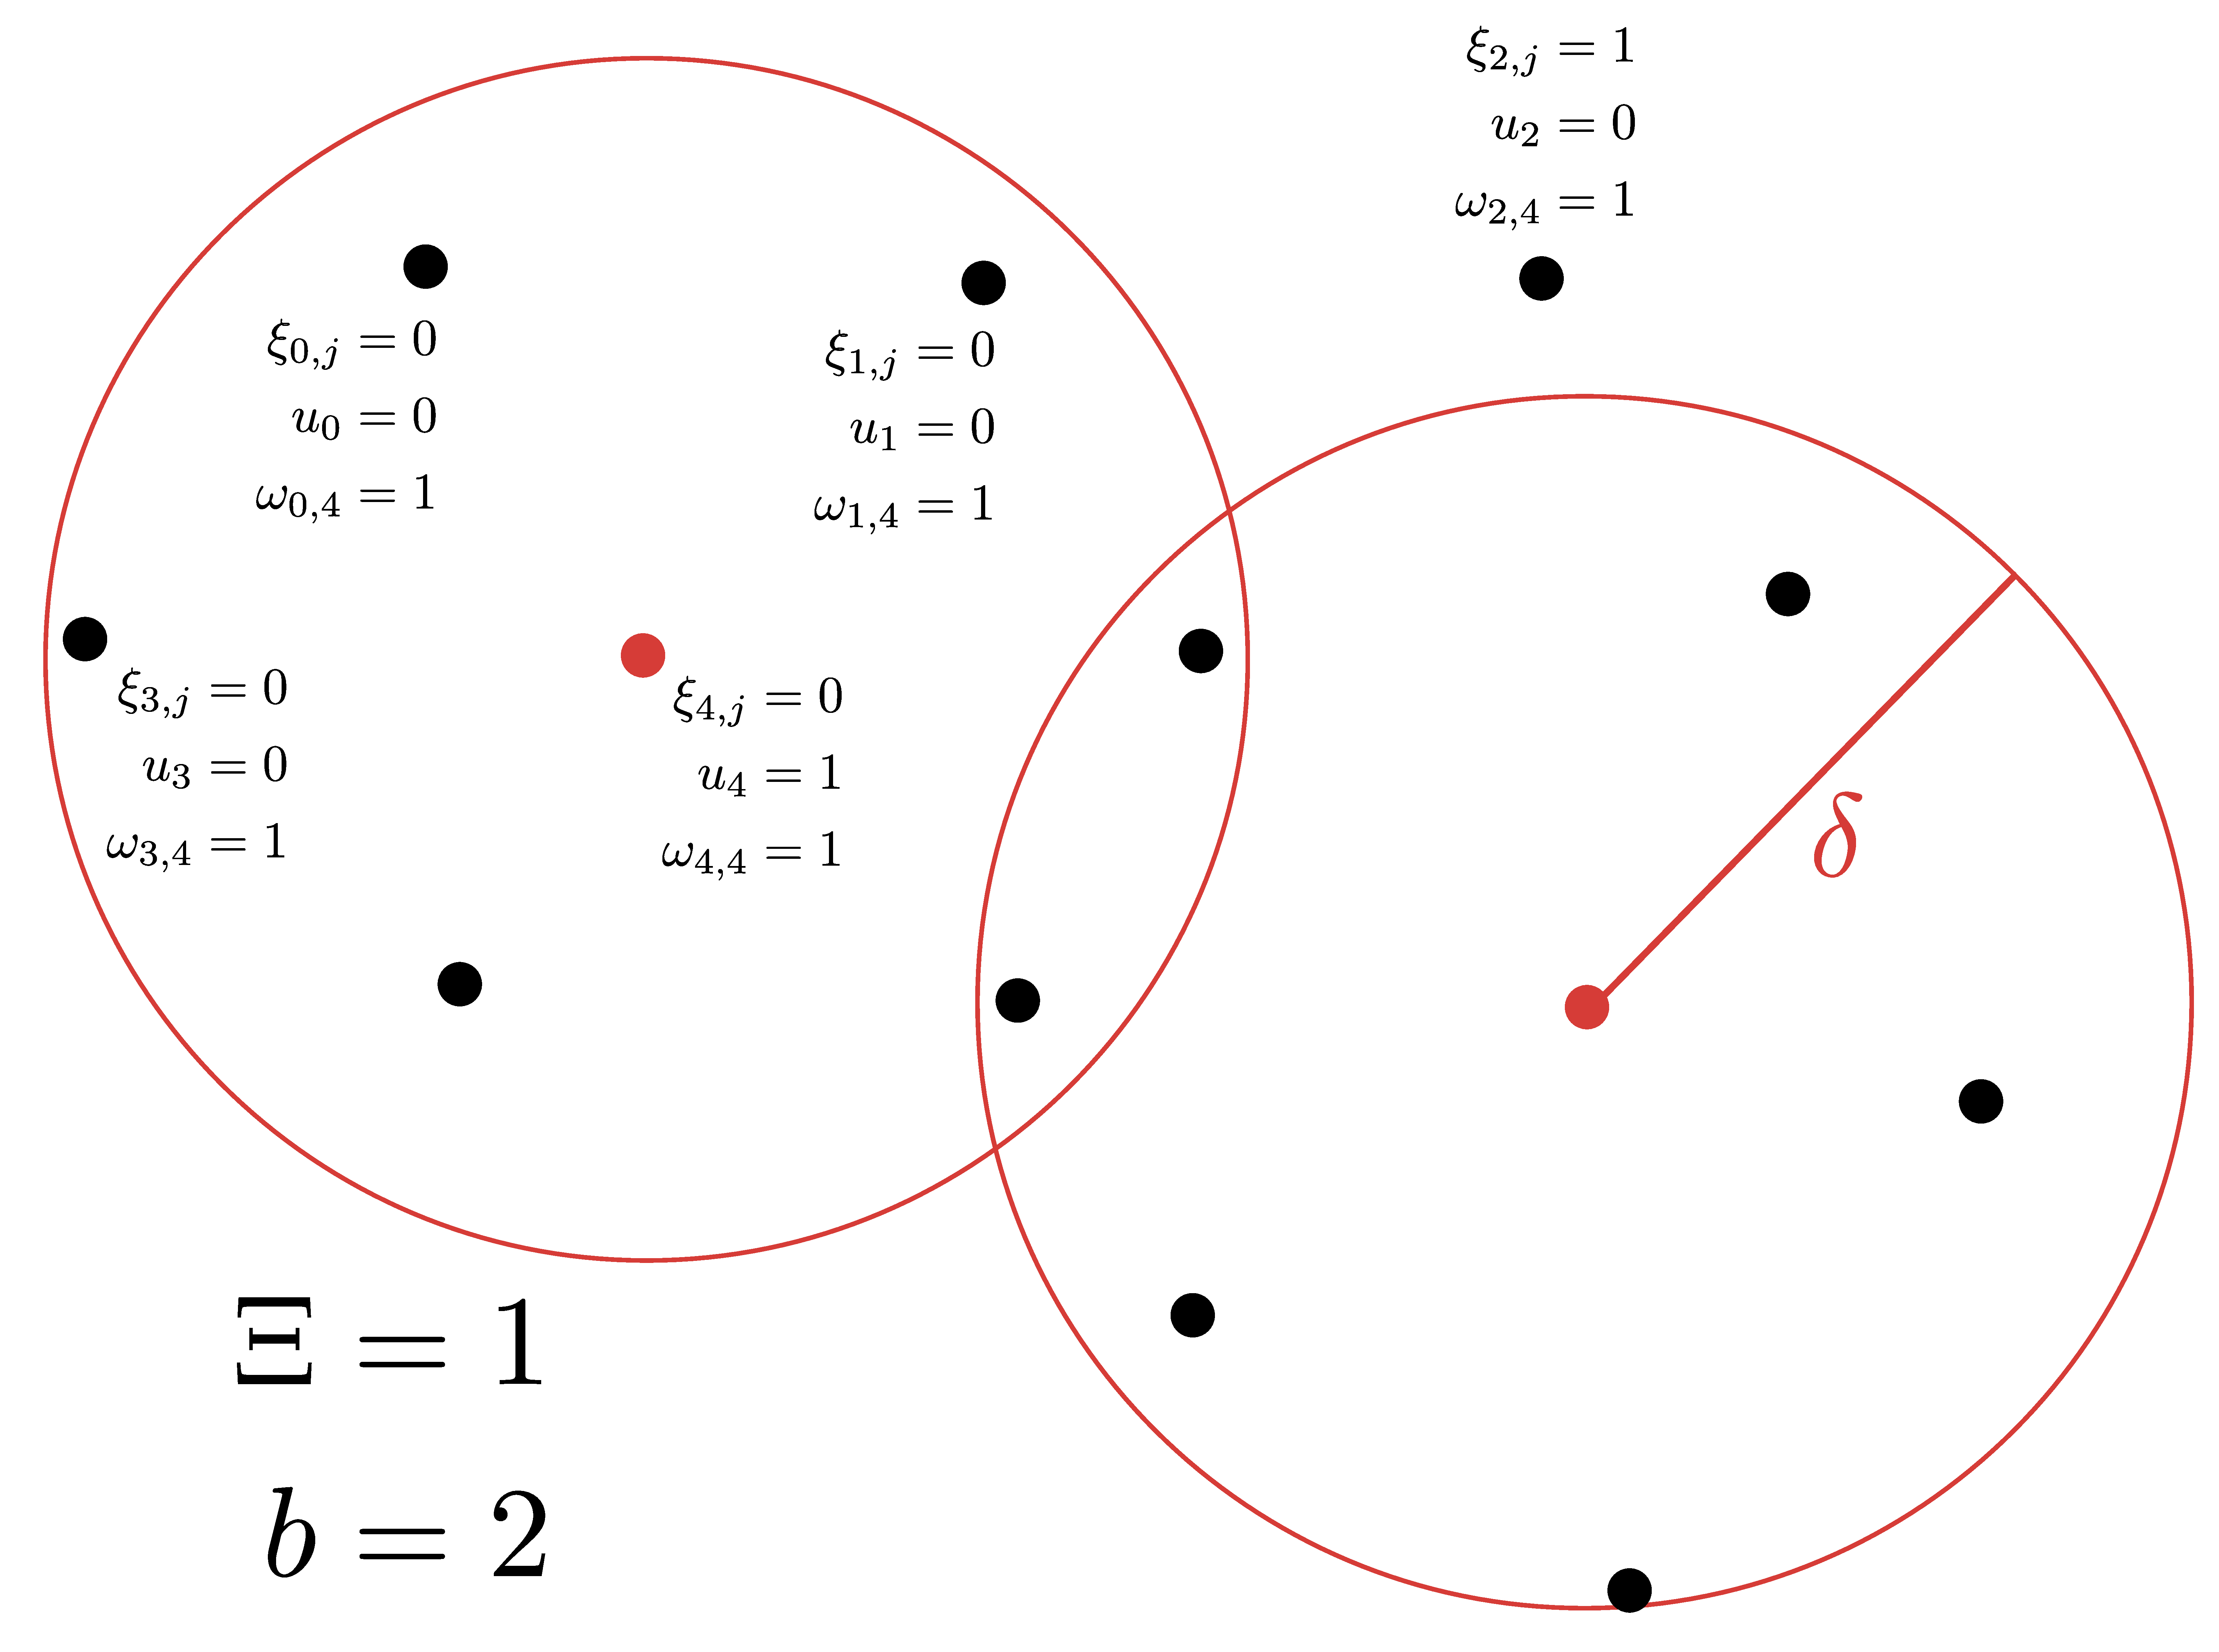
\includegraphics[width=\columnwidth]{mip.pdf}
    \caption{Visualizations of the variables in the mixed integer program. In this solution, $4^{th}$ node is chosen as a center and node $0,1,3$ is ended up in $\delta$ ball around the $4^{th}$ node. The solution also marked $2^{nd}$ node as an outlier by not including it in any $\delta$ ball.}
\label{mip}
\end{figure}


\begin{algorithm}[tb]
   \caption{Robust k-Center}
   \label{alg:bin}
\begin{algorithmic}
   \STATE {\bfseries Input:} data $\mathbf{x}_i$, existing pool $\mathbf{s}^0$, budget $b$ and outlier bound $\Xi$
   \STATE {\bfseries Initialize} $\mathbf{s}_g =$ k-Center-Greedy($\mathbf{x}_i, \mathbf{s}^0, b$)
   \STATE $\delta_{2-OPT} = \max_j \min_{i \in \mathbf{s}_g} \Delta(\mathbf{x}_i,\mathbf{x}_j)$ 
   \STATE $lb=\frac{\delta_{2-OPT}}{2}$, $ub=\delta_{2-OPT}$
   \REPEAT
   \IF {$Feasible(b, \mathbf{s}^0,\frac{lb+ub}{2},\Xi)$}
   \STATE $ub=\max_{i,j \mid  \Delta(\mathbf{x}_i,\mathbf{x}_j) \leq \frac{lb+ub}{2}}  \Delta(\mathbf{x}_i,\mathbf{x}_j) $
   \ELSE
   \STATE $lb=\min_{i,j \mid   \Delta(\mathbf{x}_i,\mathbf{x}_j) \geq \frac{lb+ub}{2}}  \Delta(\mathbf{x}_i,\mathbf{x}_j) $
    \ENDIF
   \UNTIL{$ub = lb$}
      \STATE {\bfseries return} $\{i\ st.\ u_i=1\}$
\end{algorithmic}
\end{algorithm}
\section{Implementation Details}
The distance function, semi-supervised setup etc.
We solve this mixed integer program using Gurobi\cite{gurobi} software toolbox. 
\section{Experimental Results}

\begin{figure*}
    \centering
    \begin{subfigure}[b]{0.3239\textwidth}
        
\includegraphics[width=\textwidth]{placeholder1.jpg}
        \caption{MNIST}
    \end{subfigure}
    ~ %add desired spacing between images, e. g. ~, \quad, \qquad, \hfill etc. 
      %(or a blank line to force the subfigure onto a new line)
    \begin{subfigure}[b]{0.3239\textwidth}
        
\includegraphics[width=\textwidth]{placeholder1.jpg}
        \caption{Cifar-10}
    \end{subfigure}
    ~ %add desired spacing between images, e. g. ~, \quad, \qquad, \hfill etc. 
    %(or a blank line to force the subfigure onto a new line)
    \begin{subfigure}[b]{0.3239\textwidth}
        
\includegraphics[width=\textwidth]{placeholder1.jpg}
        \caption{Cifar-100}
    \end{subfigure}
    \caption{Results on Active Learning without Semi-Supervision}\label{fig:resnosemi}
\end{figure*}

\begin{figure*}
    \centering
    \begin{subfigure}[b]{0.3239\textwidth}
        
\includegraphics[width=\textwidth]{placeholder1.jpg}
        \caption{MNIST}
    \end{subfigure}
    ~ %add desired spacing between images, e. g. ~, \quad, \qquad, \hfill etc. 
      %(or a blank line to force the subfigure onto a new line)
    \begin{subfigure}[b]{0.3239\textwidth}
        
\includegraphics[width=\textwidth]{placeholder1.jpg}
        \caption{Cifar-10}
    \end{subfigure}
    ~ %add desired spacing between images, e. g. ~, \quad, \qquad, \hfill etc. 
    %(or a blank line to force the subfigure onto a new line)
    \begin{subfigure}[b]{0.3239\textwidth}
        
\includegraphics[width=\textwidth]{placeholder1.jpg}
        \caption{Cifar-100}
    \end{subfigure}
    \caption{Results on Active Learning with Semi-Supervision}\label{fig:ressemi}
\end{figure*}


\begin{figure}[h]

\includegraphics[width=\columnwidth]{placeholder1.jpg}
\caption{Effect of approximation in set-cover problem.}
\end{figure}


\begin{figure}[h]

\includegraphics[width=\columnwidth]{placeholder1.jpg}
\caption{Test error vs $\gamma$}
\end{figure}


Lorem ipsum dolor sit amet, consectetur adipiscing elit. Sed luctus ex ac venenatis aliquam. Nulla tincidunt lacinia urna id mattis. Donec at ipsum et turpis imperdiet viverra. Etiam mauris leo, sodales iaculis maximus id, laoreet in quam. Quisque tincidunt interdum pellentesque. Cras ac odio sed urna luctus rhoncus et eu dui. Sed sem sapien, semper quis finibus nec, laoreet ac ex. Proin placerat, risus non blandit interdum, est felis condimentum erat, ac fermentum purus urna ac lacus. Curabitur sagittis turpis eu diam sodales imperdiet. Integer congue sed lacus nec tincidunt. Nam sit amet tellus quis orci dignissim aliquam condimentum sit amet risus. Etiam lectus erat, viverra eget euismod eu, tempus quis ipsum. Fusce imperdiet a purus et mollis. Morbi vulputate ante ut odio ornare, sit amet pretium ligula suscipit. Integer eu nulla cursus ligula ultrices fermentum id ut tellus.




\section{Analysis of the Algorithm}
In this section, we analyze our algorithm in terms of generalization error.  We are typically interested in the error in unseen images $E_{\mathbf{x},y \sim p_\mathcal{Z}}[l(\mathbf{x},y,A_{\mathbf{s}})]$ in terms of the empirical loss over the labelled images $\frac{1}{m}\sum_j l(\mathbf{x}_{s(i)},y_{s(i)},A_{\mathbf{s}})$. However, this analysis requires joint treatment of the generalization error and the effect of query selection. For simplicity, we divide this analysis into two parts. First, we analyze the relationship between expected loss in unseen images (generalization error) and the empirical loss over the entire dataset ($\frac{1}{n}\sum_i l(\mathbf{x}_i,y_i,A_\mathbf{s})$). Secondly, we analyze the relationship between the loss over entire dataset and empirical loss over the qeried samples. Our analysis is largely based on the gometry of the space and the geometric properties of the loss function. We rely on Lipschitz continuity of loss function and regression function. 

We study the generalization error by assuming a Lipschitz continuous loss function for a CNN. By extending the robustness results from \cite{robust}, we state the following theorem and defer its proof to the supplementary material.
\begin{theorem}
Given $n$ i.i.d. samples drawn from $p_\mathcal{Z}$ as $\{\mathbf{x}_i,y_i\}_{i\in[n]}$. If loss function $l(\cdot,y,\mathbf{w})$ is $\lambda^l$-Lipschitz continuous for all $y, \mathbf{w}$, bounded by $L$ and $\mathcal{X}x\mathcal{Y}$ has a covering number $N_{\epsilon}(\mathcal{X},|\cdot|_2)=K$; with probability at least $(1-\gamma)$,
\[
\begin{aligned}
&\left|E_{\mathbf{x},y \sim p_\mathcal{Z}}[l(\mathbf{x},y, A_\mathbf{s})] - \frac{1}{n}\sum_i l(\mathbf{x}_i,y_i,A_\mathbf{s})\right| \\
 &\hspace{3cm}\leq  \lambda^l \epsilon + L \sqrt{\frac{2K\ln 2 + 2\ln (1/\gamma)}{n}}\\
\end{aligned}
\]
\label{mainthm}
\end{theorem}

First of all, this theorem is applicable to any machine learning algorithm with Lipschitz loss function and we further prove the Lipschitz-continuity of CNNs. It can clearly be seen that the empirical loss converges to expected loss with large number of data points $n$ since $\lambda^l\epsilon$ term can be made arbitrarily small as long as $\mathcal{X}$ is a compact space. In order to complete the study about the generalization performance of CNNs, we prove the Lipschitz-continuity of the loss function of a CNN with the following lemma where max-pool and restricted liner units are the non-linearities and the loss is defined as $l_2$ distance between the desired probabilities and the soft-max outputs.

\begin{lemma}
A convolutional neural network with $n_c$ convolutional (with max-pool and ReLU) and $n_{fc}$ fully connected layers defined over C class with loss function defined as 2-norm between softmax and class probability is $\left(\frac{\sqrt{C-1}}{C} \alpha^{n_c+n_{fc}}\right)$-Lipschitz.
\end{lemma}

Here, $\alpha$ is the maximum sum of  input weights per neuron (see supplementary materials for detailed definition). Although, it is in general unbounded, it can be made arbitrarily small without changing loss function behavior (ie. keeping the label of any data point $\mathbf{s}$ unchanged) since dividing all weights with a scalar will not switch labels. Hence, for any CNN, there is equivalent CNN (in terms of classification function) with $\alpha \leq \varrho$ for any $\varrho > 0$. We can conclude that CNNs enjoy a $0$ generalization error in limiting case thanks to the Lipschitz property.

In order to complete the analysis, we need to study the behavior of the loss over the dataset in terms of the empirical loss over the selected(queried) samples. Here, we make a no training error assumption; in other words, we assume that the training error for labelled images is $0$ at the end of the learning. This is clearly a restrictive assumption; however, it is very feasible since CNNs are very representative because of their large parameter space. Moreover, this can also be easily enforced by simply converting average loss into maximal loss via \cite{maximal_loss}. We did not need this trick since our CNNs reached 0 training error in all experiments. Using this assumption, we show that the loss over the entire dataset can be bounded by the Bayes optimal classifier and the result of our discrete optimization problem.

\begin{theorem}
Given $n$ i.i.d. samples drawn from $p_\mathcal{Z}$ as $\{\mathbf{x}_i,y_i\}_{i\in[n]}$, and $m$ chosen points $\{ s(i) \in [N]\}_{\i \in [m]}$. If loss function $l(\cdot,y,\mathbf{w})$ is $\lambda^l$-Lipschitz continuous for all $y, \mathbf{w}$, regression function is $\lambda^\eta$-Lipschitz, $\{ s(i) \in [N]\}_{\i \in [m]}$ is $\delta$ cover of $\{\mathbf{x}_i,y_i\}_{i\in[n]}$, $l(\mathbf{x}_{s(j)},y_{s(j)},A_\mathbf{S})=0\quad \forall j \in [m]$; with probability at least $1-\gamma$,
\begin{small}
\[
\frac{1}{n}\sum_i l(\mathbf{x}_i,y_i,A_\mathbf{s}) \leq \mathcal{L}_{[n]} (h^\star) +\delta(\lambda^l + 2 \lambda^{\eta}) + 
\sqrt{\frac{\log(1/1-\gamma)}{2n}}
\]
\end{small}
where $\mathcal{L}_{[n]} (h^\star)$ is the loss of the Bayes-optimal classifier.
\label{mainthm2}
\end{theorem}

It can easily be shown that; in this setting, $\lim_{n \rightarrow \infty} \frac{1}{n}\sum_i l(\mathbf{x}_i,y_i,A_\mathbf{s}) =   \mathcal{L}_{[n]} (h^\star) +\delta(\lambda^l + 2 \lambda^{\eta})$. Clearly, $\delta$ decreases when $m$ increases; however, the rate is critical. To show that our algorithm sounds, we need to show that $\delta$ can be made arbitrarily small with finite $m$ in the limiting behavior of number of unlabelled data points (i.e. $n \rightarrow \infty$). Since our data points are coming from a compact space, there exist a finite sub-cover to any union of open sets. Hence, the finite query property is straightforward result of compactness. We give the following corollary without proof;

\begin{cor}
Given $n$ i.i.d. samples drawn from $p_\mathcal{Z}$ as $\{\mathbf{x}_i,y_i\}_{i\in[n]}$, and a desired error rate $\rho$. If loss function $l(\cdot,y,\mathbf{w})$ is $\lambda^l$-Lipschitz continuous for all $y, \mathbf{w}$, regression function is $\lambda^\eta$-Lipschitz, there exist a finite subset $\mathbf{s}$ with cardinality m such that any CNN achieving $0$ error over $\{\mathbf{x}_{s(j)},y_{s(j)}\}_{j \in [m]}$ achieve the following with probability $1$.
\[
\lim_{n \rightarrow \infty} \frac{1}{n}\sum_i l(\mathbf{x}_i,y_i) \leq \mathcal{L}_{[n]} (h^\star) +\rho
\]
where $\mathcal{L}_{[n]} (h^\star)$ is the loss of the Bayes-optimal classifier.
\label{maincor}
\end{cor}

In summary, we show that CNNs have Lipschitz continuous loss functions, making them generalizes to unseen images. In addition, when the underlying data distribution has Lipschitz continuous regression functions, we further show, under reasonable assumptions, a small subset of dataset is enough to be labelled as long as it covers the space efficiently. Consider the fact that the difference between the empirical loss over unseen images and the optimal loss is bounded by $\delta(\lambda^l + 2 \lambda^{\eta})$. Moreover, our algorithm is based on direct minimization of $\delta$. Hence, our proposed method directly minimizes this loss and theoretical analysis validates our space-covering heuristic.

\section{Conclusion}
Suspendisse pharetra erat sapien, sit amet porta mi cursus congue. Sed pulvinar justo in metus sollicitudin mollis. Mauris sagittis dui vitae arcu gravida, et lacinia mauris ultrices. Sed faucibus nibh ac velit vehicula, ac molestie tellus mattis. Duis nec tellus erat. Aliquam pellentesque nibh quis ex blandit euismod porta id leo. In facilisis finibus nisl, rhoncus dignissim dui lobortis sit amet. Nulla pellentesque, nisi ac porta consectetur, lorem nisl rhoncus dolor, sed ornare mi nisi maximus magna. Integer nunc ipsum, lobortis vel diam in, vestibulum iaculis felis. Etiam viverra fermentum scelerisque. Praesent facilisis ultrices magna, sit amet dignissim velit rutrum tempor. Nunc in diam elit. Vestibulum eget molestie erat. 

\bibliography{active_adversarial} 
\bibliographystyle{icml2017}


\begin{proof}
It is easy to show that for any differentiable function $f:\mathbb{R}^n\rightarrow\mathbb{R}^m$,

\[
\left \|f(x)-f(y)\right \|_2 \leq \left \|J\right \|^*_F \left \|x-y\right\|_2 \, \, \forall x,y\in\mathbb{R}^n
\]
where $\left \|J\right \|^*_F = \max\limits_{x} \left \|J\right \|_F$ and $J$ is the jacobian matrix of $f(x)$ wrt $x$.

Softmax function is defined as
\[
f(x)_i = \frac{\exp(x_i)}{\sum\limits_{j=1}^{C}\exp(x_j)} = p_i(x), \, i={1,2,...C}
\]
For brevity, We will denote $p_i(x)$ as $p_i$. The jacobian matrix for some $x$ will be,
\[
J = \begin{bmatrix} p_1(1-p_1) & p_1p_2  & ... & p_1p_K \\
p_2p_1 & p_2(1-p_2)  & ...  & p_2p_K \\
... & ... & ... & ...  \\
p_{K}p_{1} & p_{K}p_{2}  & ...  & p_{K}(1-p_{K})
\end{bmatrix}
\]
Now, Frobenius norm of above matrix will be,
\[
\left \| J \right \|_F = \sqrt{\sum\limits_{i=1}^{K}\sum\limits_{j=1 \\ i\neq j}^{K}p_{i}^{2}p_{j}^{2} + \sum\limits_{i=1}^{K} p_i^2(1-p_i^2)}
\]
It is straightforward to show that $p_i = \frac{1}{K}$ is the optimal solution for $\left \| J \right \|^{*}_F = \max\limits_{x}\left \| J \right \|_F $ Hence,


Putting $p_i = \frac{1}{K}$ in above equation of $\left \| J \right \|_F$, we get $\left \| J \right \|^{*}_F = \frac{\sqrt{K-1}}{K}$

\end{proof}


\begin{proof}
Consider two inputs $\mathbf{x}_u$ and $\mathbf{x}_v$, such that their representation at layer $d$ is $\mathbf{x}_u^d$ and $\mathbf{x}_v^d$. Consider any conv+max pool+relu layer, if $\sum_i w_{i,j} \leq \alpha \forall j$, we can simply state
\[
|\mathbf{x}_u^d - \mathbf{x}_v^d| \leq  \alpha |\mathbf{x}_u^{d-3} - \mathbf{x}_v^{d-3}|
\] 
Here, we used $|a-b| \leq |\max(0, a) - \max(0,a)|$ and the fact that max pool layer can be written as a convolutional layer such that only one weight is 1 and others are 0. For fully connected layers, we can also use the same argument and show;
\[
|\mathbf{x}_u^d - \mathbf{x}_v^d| \leq  \alpha |\mathbf{x}_u^{d-1} - \mathbf{x}_v^{d-1}|
\] 
For soft-max layer, we need to use the Lemma \ref{softmax_lip} as,
\[
|\mathbf{x}_u^d - \mathbf{x}_v^d| \leq  \frac{\sqrt{C-1}}{C} |\mathbf{x}_u^{d-1} - \mathbf{x}_v^{d-1}|
\] 
Hence,
\[
|l(\mathbf{x}_u) - l(\mathbf{x}_v)| \leq   \frac{\sqrt{C-1}}{C} \alpha^{n_c+n_{fc}}  |\mathbf{x}_u-\mathbf{x}_v|
\]
\end{proof}

\begin{proof}
\begin{small}
We will start with
\[
\begin{aligned}
&\left|E[l(x,y)] - \frac{1}{n}\sum_i l(x_i,y_i) \right| \\
&\leq \left|\sum_{j} E[l(x,y)| (x,y) \in C_j] \mu_{j} -  \sum_{j} E[l(x,y)| (x,y) \in C_j] \frac{|N_j|}{n} \right| \\
 &+  \left|\sum_{j} E[l(x,y)| (x,y) \in C_j] \frac{|N_j|}{n}  - \frac{1}{n}\sum_i l(x_i,y_i)\right| \\
  &\leq\left|\sum_{j} E[l(x,y)| (x,y) \in C_j] (\mu_{j} -   \frac{|N_j|}{n}) \right|\\
 &+\frac{1}{n} \left|\sum_j \sum_{i \in N_j} E[l(x,y)| (x,y) \in C_j]  - l(x_i,y_i)\right| \\
   &\leq \left|\sum_{j} E[l(x,y)|z \in C_j] (\mu_{j} -   \frac{|N_j|}{n})\right| + \lambda^l \epsilon^s  \\
 \end{aligned}
\]
%Now, we will use the zero-loss of the classifier with Lipschitz continuity as;
%\[
%\begin{aligned}
%\left|\frac{1}{n}\sum_i l(A_s,x_i) \right| &= \left|\frac{1}{n}\sum_{j \notin {s(i)}_{i\in [M]}} l(A_s,x_i)  \right| \\
%&\leq  \frac{1}{n}\sum_{j \notin {s(i)}_{i\in [M]}} \lambda  \left| \mathbf{x}_i - \mathbf{x}_k\right | \leq \frac{n-m}{n} \lambda \tilde{\epsilon}
%\end{aligned}
%\]
%Combining both,
%\[
%\begin{aligned}
%&E[l(A_s,z)] \leq  \left|E[l(A_s,z)] - \frac{1}{n}\sum_i l(A_s,x_i) \right|  \\ &+ \left|\frac{1}{n}\sum_i l(A_s,x_i) - \frac{1}{m}\sum_i l(A_s,x_{s(i)}) \right| \\
%&\leq \left|\sum_{j} E[l(A_s,z)|z \in C_j] (\mu_{j} -   \frac{|N_j|}{n})\right| +\epsilon(s) + \frac{n-m}{n} \lambda \tilde{\epsilon}
%\end{aligned}
%\]
\end{small}
We finally use Breteganolle-Huber-Carol inequality (\emph{cf} Proposition A6.6 of \cite{wellner}):
\[
\left| E[l(x,y)] - \frac{1}{n}\sum_i l(x_i,y_i) \right| \leq \lambda^l \epsilon^s + L \sqrt{\frac{2K\ln 2 + 2\ln (1/\gamma)}{n}}
\]
\end{proof}

\begin{lemma}
For $\mathbf{x}_i, \mathbf{x}_j$ such that $|\mathbf{x}_i -\mathbf{x}_j|\leq \epsilon$ and $\eta_c(x)$ is $\lambda^\eta$-Lipschitz and $l(\cdot,y)$ is $\lambda^l$-Lipschitz,
\[
E[|l(\mathbf{x_2},y_2) -l(\mathbf{x_1},y_1)|] \leq  \epsilon(\lambda^l + 2 \lambda^{\eta}) + E[l(h^\star)]
\]
\end{lemma}
\begin{proof}
Without loss of generality, assume $y_1=c$, then 
\[
\begin{aligned}
p(y_1 \neq y_2)&=p(y_2 \neq c)\\
&= p_{y_2 \sim \eta_c(\mathbf{x}_2)}(y_2\neq c)
\\&\leq p_{y_2 \sim \eta_c(\mathbf{x}_1)}(y_2 \neq c) + |\eta_c(\mathbf{x}_1) - \eta_c(\mathbf{x}_2)|\\
&\leq 1 - \eta_{y_1}(\mathbf{x_1}) + \lambda^{\eta}\epsilon
\end{aligned}
\]
then we use this in the following
\[
\begin{aligned}
&E[|l(\mathbf{x_2},y_2) -l(\mathbf{x_1},y_1)|] \\ &= E[|l(\mathbf{x_2},y_2) -l(\mathbf{x_1},y_1)||y_1=y_2] p(y_1=y_2) \\ &\quad+ E[|l(\mathbf{x_2},y_2) -l(\mathbf{x_1},y_1)||y_1\neq y_2] p(y_1 \neq y_2) \\
&\leq \lambda^l \epsilon p(y_1=y_2) + 2 p(y_1 \neq y_2)\\
&\leq \lambda^l \epsilon + 2(1 - \eta_{y_1}(\mathbf{x_1}) + \lambda^{\eta}\epsilon) \\
&= \epsilon(\lambda^l + 2 \lambda^{\eta}) + E[l(h^\star)]
\end{aligned}
\]
\end{proof}

\begin{proof}
We need to bound the empirical risk of the unlabelled images,
\[
\begin{aligned}
E[ l(\mathbf{x}_i,y_i)] &= E[ l(\mathbf{x}_i,y_i) - l(\mathbf{x}_k,y_k) ] \\ 
&\leq \epsilon(\lambda^l + 2 \lambda^{\eta}) + E[l(h^\star)]
\end{aligned}
\]
We further use the Hoeffding's Bound and conclude that with probability at least $1 - \delta$,
\[
\frac{1}{n}\sum_i l(\mathbf{x}_i,y_i) \leq E[l(h^\star)] +\epsilon(\lambda^l + 2 \lambda^{\eta}) + 
\sqrt{\frac{\log(1/1-\delta)}{2n}}
%\frac{\log(1/(1-\delta)){2n}
\]
\end{proof}

\begin{lemma}
Softmax function defined over $C$ class is  Lipschitz continuous with $\lambda=\frac{\sqrt{C-1}}{C}$
\end{lemma}


\begin{cor}
If the conditions in Theorem \ref{mainthm} satisfied except $4$ and $l_{emp}(A_s,x)=0\quad \forall x \in \overline{s}$, with probability at least $(1-\gamma)$,
\begin{small}
\[
E[l(A_s,z)] \leq \frac{n-|\overline{s}|}{n} \lambda \tilde{\epsilon} + \epsilon(s) + L \sqrt{\frac{2K\ln 2 + 2\ln (1/\gamma)}{n}} + \frac{2|s|L}{n}  
\]
\end{small}
\end{cor}
\begin{proof}
\[
\begin{aligned}
&\left|\frac{1}{n}\sum_i l(A_s,x_i) \right| \leq \left|\frac{1}{n}\sum_{j \notin {s(i)}_{i\in [M]}} l(A_s,x_i)  \right| +  \left|\frac{1}{n}\sum_{j \notin\overline{s}} l(A_s,x_i)  \right| \\
&\leq  \frac{1}{n}\sum_{j \notin {s(i)}_{i\in [M]}} \lambda  \left| \mathbf{x}_i - \mathbf{x}_k\right | +\frac{n-|\overline{s}|}{n}L \\
&\leq \frac{n-m}{n} \lambda \tilde{\epsilon}
\end{aligned}
\]
\end{proof}

\end{document} 
